\def\problemCode{\LR{inversions}}
\def\problemFarsiTitle{نابه‌جایی}

\begin{problem}

  مسئله شمردن تعداد نابه‌جایی‌های یک جایگشت را در نظر بگیرید.
  تعداد نابه‌جایی‌های جایگشت 
  $p$
  برابر تعداد زوج مرتب‌های
  $i < j$
  است که
  $p_i > p_j$
  .
  تعداد نابه‌جایی‌ها را می‌توانیم با استفاده از الگوریتم
  \LR{merge sort}
  در زمان
  $\mathcal{O}(n \, log \, n)$
  پیدا کنیم، اما به دنبال راه دیگری برای حل آن هستیم.

  برای عضو
  $i$
  -
  ام جایگشت یک نقطه در فضای دوبعدی در جایگاه
  $(i, p_i)$
  رسم می‌کنیم.
  روشن است که 
  تعداد نابه‌جایی‌های جایگشت
  $p$
  با تعداد زوج نقطه‌هایی که 
  نقطه‌ی سمت راست‌تر، پایین‌تر نیز می‌باشد، برابر است.

  \begin{center}
    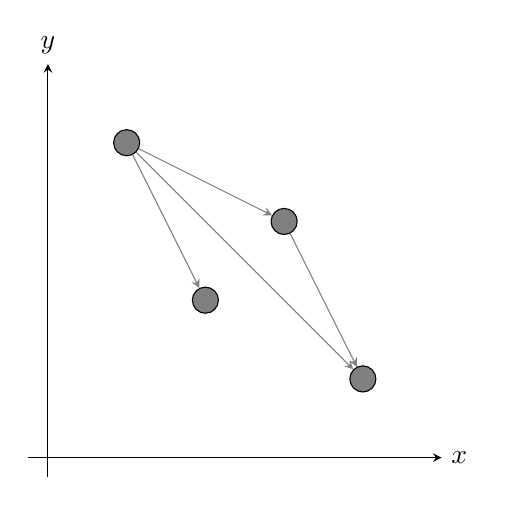
\begin{tikzpicture}[x=1cm, y=1cm, >=stealth]
        \draw[->] (-0.25,0) -- (5,0)
            node [right] {$x$};
        \draw[->] (0,-0.25) -- (0,5)
            node [above] {$y$};
        
        \node[fill=gray, circle, draw] (1) at (1,4) {};
        \node[fill=gray, circle, draw] (2) at (2,2) {};
        \node[fill=gray, circle, draw] (3) at (3,3) {};
        \node[fill=gray, circle, draw] (4) at (4,1) {};

        \draw [->, gray] (1) -- (2);
        \draw [->, gray] (1) -- (3);
        \draw [->, gray] (1) -- (4);
        \draw [->, gray] (3) -- (4);
    \end{tikzpicture}
    \captionof{figure}{نقاط و نابه‌جایی‌های جایگشت
    $p = \langle 4, 2, 3, 1 \rangle$
    } 
    \label{fig:your Label}
\end{center}

  تکنیکی که در این مسئله استفاده می‌کنیم، 
  خطی عمودی فرضی‌ای است که از
  $x = -\infty$
  شروع می‌شود و به سمت
  $x = \infty$
  حرکت می‌کند.
  به نقاط یک لامپ وصل می‌کنیم و 
  در ابتدا همه‌ی آن‌ها را خاموش فرض می‌کنیم.
  خط فرضی از روی هر نقطه‌ای که گذر کند، 
  لامپ آن نقطه روشن می‌شود.
  می‌توانید حدس بزنید که وقتی خط فرضی به 
  $x$
  نقطه‌ای می‌رسد، 
  چگونه می‌توانیم نقاطی را پیدا کنیم 
  که سمت چپ و بالای نقطه فرض شده باشد.

  در واقع با استفاده از تکنیک لامپ خاموش و روشن، 
  وقتی به نقطه‌ای می‌رسیم، تنها لامپ نقاطی روشن است 
  که سمت چپ آن باشند. انگار که یکی از شرط‌های
  $x_1 < x_2$
  و
  $y_1 < y_2$
  را با استفاده از این تکنیک مدیریت کرده‌ایم و 
  تنها کافی است که تعداد نقاط روشن
  $i$
  را پیدا کنیم که
  $y_i > y_{now}$
  هستند.

  در اکثر مواقع این بخش از مسئله با استفاده از 
  \LR{Segment Tree}
  قابل حل است. در این مثال وقتی لامپ نقطه‌ی 
  $(x, y)$
  را روشن می‌کنیم،
  از سگمنت می‌خواهیم
  مقدار خانه
  $y$
  را با 
  $+1$
  جمع بزند.
  و وقتی می‌خواهیم تعداد نقاط سمت چپ و بالای نقطه
  $(x, y)$
  را پیدا کنیم،
  هنگامی که خط فرضی به 
  $x$
  رسید،
  جمع بازه‌ی 
  $[y + 1, \infty]$
  را از سگمنت دریافت می‌کنیم.

  پس با سگمنتی که دو عملیات زیر را انجام می‌دهد، مسئله را حل کردیم.
  \begin{enumerate}
    \item
      مقدار خانه
      $idx$
      را با
      $value$
      جمع بزن.
    
    \item
      جمع بازه‌ی
      $L$
      تا
      $R$
      از آرایه چند است؟
  \end{enumerate}
\end{problem}
